\documentclass[tikz]{standalone}
\usetikzlibrary{arrows.meta, positioning}
\begin{document}
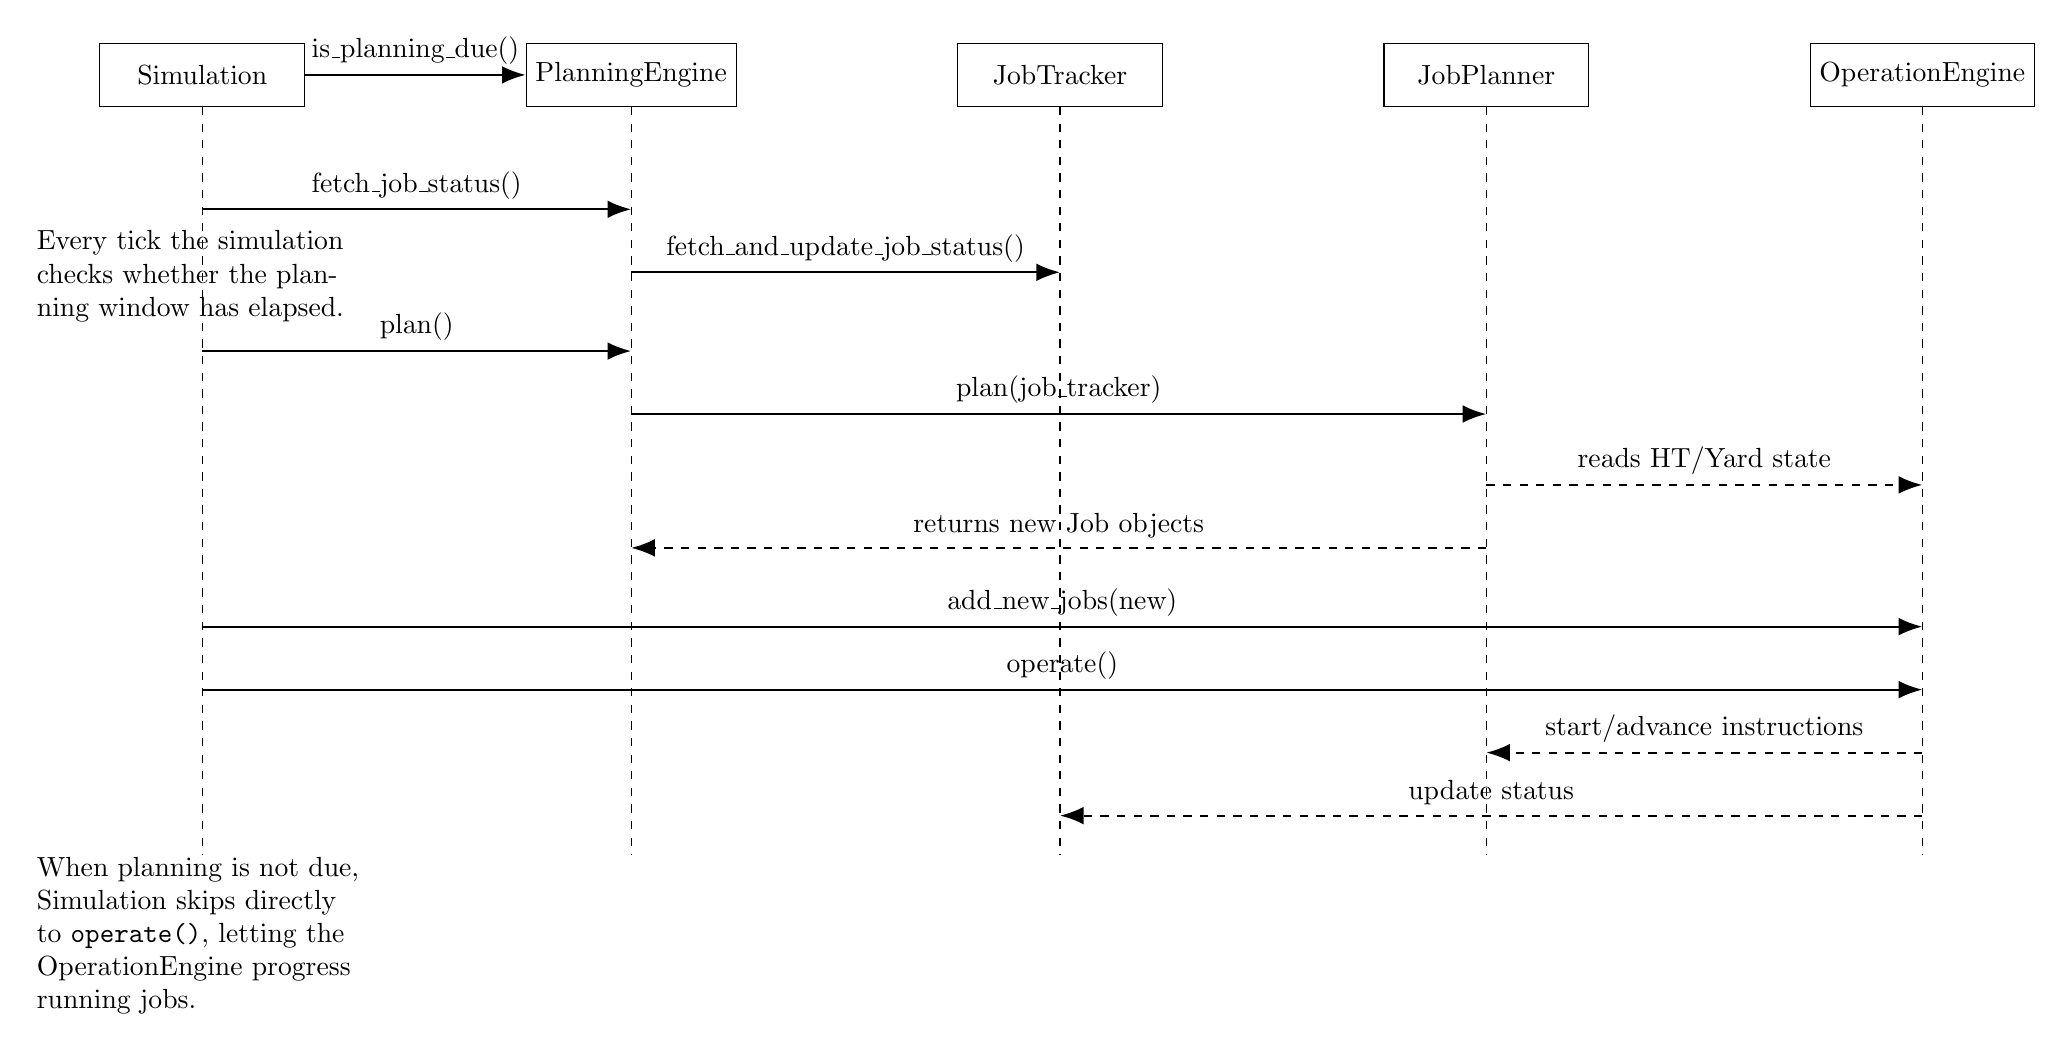
\begin{tikzpicture}[
    lifeline/.style={draw, minimum width=2.6cm, minimum height=0.8cm, align=center},
    call/.style={-{Latex[length=3mm]}, thick},
    dashedcall/.style={-{Latex[length=3mm]}, thick, dashed},
    note/.style={align=left, text width=4.2cm},
    node distance=1.2cm
]
    % Lifelines
    \node[lifeline] (sim) {Simulation};
    \node[lifeline, right=2.8cm of sim] (planeng) {PlanningEngine};
    \node[lifeline, right=2.8cm of planeng] (jobtracker) {JobTracker};
    \node[lifeline, right=2.8cm of jobtracker] (jobplanner) {JobPlanner};
    \node[lifeline, right=2.8cm of jobplanner] (openg) {OperationEngine};

    % Lifeline lines
    \draw[dashed] (sim.south) -- +(0,-9.5);
    \draw[dashed] (planeng.south) -- +(0,-9.5);
    \draw[dashed] (jobtracker.south) -- +(0,-9.5);
    \draw[dashed] (jobplanner.south) -- +(0,-9.5);
    \draw[dashed] (openg.south) -- +(0,-9.5);

    % Sequence of calls
    \node[below=1.1cm of sim] (tickstart) {};

    \draw[call] (sim) -- node[above]{is\_planning\_due()} (planeng);
    \node[note, below=0.1cm of tickstart] {Every tick the simulation checks whether the planning window has elapsed.};

    \draw[call] ([yshift=-1.3cm]sim.south) -- node[above]{fetch\_job\_status()} ([yshift=-1.3cm]planeng.south);
    \draw[call] ([yshift=-2.1cm]planeng.south) -- node[above]{fetch\_and\_update\_job\_status()} ([yshift=-2.1cm]jobtracker.south);

    \draw[call] ([yshift=-3.1cm]sim.south) -- node[above]{plan()} ([yshift=-3.1cm]planeng.south);
    \draw[call] ([yshift=-3.9cm]planeng.south) -- node[above]{plan(job\_tracker)} ([yshift=-3.9cm]jobplanner.south);
    \draw[dashedcall] ([yshift=-4.8cm]jobplanner.south) -- node[above]{reads HT/Yard state} ([yshift=-4.8cm]openg.south);
    \draw[dashedcall] ([yshift=-5.6cm]jobplanner.south) -- node[above]{returns new Job objects} ([yshift=-5.6cm]planeng.south);

    \draw[call] ([yshift=-6.6cm]sim.south) -- node[above]{add\_new\_jobs(new)} ([yshift=-6.6cm]openg.south);
    \draw[call] ([yshift=-7.4cm]sim.south) -- node[above]{operate()} ([yshift=-7.4cm]openg.south);
    \draw[dashedcall] ([yshift=-8.2cm]openg.south) -- node[above]{start/advance instructions} ([yshift=-8.2cm]jobplanner.south);
    \draw[dashedcall] ([yshift=-9.0cm]openg.south) -- node[above]{update status} ([yshift=-9.0cm]jobtracker.south);

    \node[note, below=9.4cm of sim] {When planning is not due, Simulation skips directly to \texttt{operate()}, letting the OperationEngine progress running jobs.};
\end{tikzpicture}
\end{document}
